\documentclass[%
 aip,
 jcp,
 amsmath,amssymb,
 preprint,%
%reprint,%
]{revtex4-1}


\usepackage{graphicx}
\usepackage{dcolumn}
\usepackage{bm}
\usepackage[utf8]{inputenc}
\usepackage[T1]{fontenc}

\usepackage{tikz}

\usepackage{xr}
%\externaldocument[SI-]{si}


\begin{document}

\title{Hierarchical Bayesian calibration of mesoscopic models for ultrasound contrast agents from force spectroscopy data}

\author{Brieuc Benvegnen}
\thanks{These authors contributed equally to this work.}
\affiliation{Universitat de Barcelona Institute of Complex Systems (UBICS),
C/ Martí i Franqués 1, 08028 Barcelona, Spain}

\author{Nikolaos Ntarakas}
\thanks{These authors contributed equally to this work.}
\affiliation{Theory Department, National Institute of Chemistry,
Hajdrihova 19, 1001 Ljubljana, Slovenia}
\affiliation{Department of Physics, Faculty of Mathematics and Physics,
University of Ljubljana, Jadranska 19, 1000 Ljubljana, Slovenia}

\author{Tilen Potisk}
\affiliation{Theory Department, National Institute of Chemistry,
Hajdrihova 19, 1001 Ljubljana, Slovenia}
\affiliation{Department of Physics, Faculty of Mathematics and Physics,
University of Ljubljana, Jadranska 19, 1000 Ljubljana, Slovenia}

\author{Ignacio Pagonabarraga}
\affiliation{Universitat de Barcelona Institute of Complex Systems (UBICS),
C/ Martí i Franqués 1, 08028 Barcelona, Spain}

\author{Matej Praprotnik}
\email[Author to whom correspondence should be addressed: ]{praprot@cmm.ki.si}
\affiliation{Universitat de Barcelona Institute of Complex Systems (UBICS),
C/ Martí i Franqués 1, 08028 Barcelona, Spain}
\affiliation{Theory Department, National Institute of Chemistry,
Hajdrihova 19, 1001 Ljubljana, Slovenia}
\affiliation{Department of Physics, Faculty of Mathematics and Physics,
University of Ljubljana, Jadranska 19, 1000 Ljubljana, Slovenia}

\begin{abstract}
Ultrasound-guided drug and gene delivery (\textsc{usdg}) is a promising non-invasive approach for targeted therapeutic applications. Mechanical properties of encapsulated microbubbles (\textsc{emb}s), which serve as contrast agents, affect their interactions with ultrasound and are thus critical to the success of \textsc{usdg}. Accurate calibration of particle-based \textsc{emb} models is challenging as Bayesian inference with dissipative particle dynamics (\textsc{dpd}) is prohibitively computationally expensive. We employ a surrogate-accelerated Bayesian calibration workflow that combines deep neural network (\textsc{dnn}) surrogates and polynomial surrogates, transitional Markov chain Monte Carlo sampling, and hierarchical regularization across \textsc{emb} diameters. Using this framework, we construct data-informed models of the commercial agents Definity and SonoVue, and infer their force field parameters from published compression, indentation, and acoustic experiments. The presented methodology can be used to derive bespoke, data-informed models for a wide range of contrast agents, including gas vesicles, \textsc{emb}s with diverse capsids consisting of lipids, proteins, or polymers, and functionalized with ligands.
\end{abstract}

\maketitle

\section{Introduction}

Encapsulated microbubbles (\textsc{emb}s) are a class of engineered soft materials with gas cores surrounded by elastic shells, composed of a lipid, protein or polymer shell and typically 1 to 10\,\textmu m in diameter~\citep{stride2009physical,ferrara2007ultrasound}. These structures serve dual roles in biomedical applications: as ultrasound contrast agents that enhance diagnostic imaging through acoustic scattering~\citep{klibanov2006microbubble,datta2008ultrasound}, and as targeted drug delivery vehicles capable of payload release upon ultrasonic excitation~\citep{ferrara2007ultrasound,sirsi2014state,stride2010cavitation,coussios2008applications}. The mechanical properties of \textsc{emb} shells, particularly their elastic modulus, bending rigidity, and response to compression, critically determine bubble stability under physiological flow conditions, acoustic response, and rupture thresholds for controlled drug release~\citep{stride2009physical,guo2013investigation,stride2010cavitation,konofagou2012optimization}. Accurate characterization of these mechanical properties enables rational design of \textsc{emb}s optimized for specific clinical applications, including targeted chemotherapy delivery to tumor vasculature~\citep{tinkov2009microbubbles,tinkov2010new} and blood--brain barrier permeabilization for neurotherapeutics~\citep{hynynen2001noninvasive}. However, systematic quantification of \textsc{emb} mechanical parameters with rigorous uncertainty bounds remains an open challenge, limiting predictive modeling of \textsc{emb} behavior in complex in vivo environments.

Experimental characterization of \textsc{emb} mechanical properties typically employs atomic force microscopy (\textsc{afm}) compression~\citep{glynos2009polymeric,glynos2009nanomechanics}, micropipette aspiration~\citep{evans1989aspiration} or ultrasonic attenuation measurements~\citep{church1995effects,coussios2008applications}. \textsc{afm} compression provides direct force-displacement relationships at nanometer resolution but is subject to experimental uncertainties, including contact point determination, tip-sample alignment artifacts, and batch-to-batch variability in \textsc{emb} synthesis~\cite{glynos2009nanomechanics,tu2009estimating}. Translating these force-displacement curves into fundamental material properties (e.g., Young's modulus, bending modulus) requires computational models that can simulate \textsc{emb} deformation under realistic experimental conditions. Continuum models based on finite element methods offer computational efficiency and have been widely used to model \textsc{emb} dynamics in fluid and vascular environments~\citep{zhang2018mechanics,guo2024ultrasound}, but make strong assumptions about shell constitutive behavior (e.g., Neo-Hookean elasticity) and cannot capture heterogeneities at the molecular scale of shell composition. Particle-based mesoscopic simulations, particularly dissipative particle dynamics (\textsc{dpd}), provide a complementary approach that explicitly represents the shell microstructure through coarse-grained particles interacting via prescribed force fields~\citep{groot1997dissipative,espanol1995statistical}. Our previous work demonstrated that \textsc{dpd} models with isotropic elasticity and bending resistance can accurately reproduce \textsc{emb} compression behavior across multiple shell-chemistry compositions~\citep{ntarakas2025dissipative}. However, \textsc{dpd} simulations require 30--60 minutes per parameter configuration on modern \textsc{gpu}s (e.g. \textsc{nvidia} A40), making systematic parameter space exploration prohibitively expensive. A single Bayesian inference run that requires $10^5$ likelihood evaluations would already consume roughly $3\times10^{6}$-- $6\times10^{6}$~\textsc{gpu}-minutes, i.e. about 5.7--11.4 \textsc{gpu}-years, even before accounting for repeated phases, restarts, or the one-time generation of surrogate-training data, making direct \textsc{dpd}-based Bayesian uncertainty quantification intractable in the present setup.
\textsc{uq} constitutes a framework for addressing imperfections in models, simulations, and experimental data \citep{angelikopoulos2012bayesian}. By representing unknown parameters and model discrepancies as distributions instead of fixed values, \textsc{uq} enables predictions that reflect both expected behavior and associated confidence, which is essential for making reliable, data-informed decisions in complex systems. Bayesian inference serves as a framework for \textsc{uq} through parameter estimation with quantified uncertainties~\citep{gelman2013bayesian,gregory2005bayesian,nordman2025bayesian,amoudruz2025bayesian}, transforming point estimates into probability distributions that capture both data informativeness and prior knowledge. Hierarchical Bayesian \textsc{uq} extends this framework to settings with multiple datasets or experimental conditions, allowing parameters to vary across conditions while sharing a common structure \citep{wu2016fusing}. This enables information sharing, improves parameter identifiability, and yields a more realistic representation of variability in complex systems. In molecular and mesoscopic simulations, Bayesian approaches have been used to calibrate force fields for proteins~\citep{cailliez2014calibration}, polymers~\citep{zhang2014polymer}, and soft materials~\citep{angelikopoulos2012bayesian}. The computational bottleneck of repeated forward model evaluations can be mitigated with surrogate modeling, using fast approximations such as Gaussian processes, neural networks, or polynomial chaos expansions that learn input-output relationships from a limited training dataset~\citep{rasmussen2006gaussian,wu2022multi}. Deep neural network (\textsc{dnn}) surrogates are particularly attractive for high-dimensional nonlinear systems because they can reproduce complex input-output maps with large speedups over direct simulation~\citep{raissi2019physics,lu2021deepxde}. Bayesian optimization has also emerged as an efficient strategy for refining model parameters in computationally expensive settings, where each evaluation requires a forward simulation \citep{ray2025refining}. By combining a surrogate model with an acquisition function, it enables adaptive exploration of the parameter space and rapid identification of optimal coarse-grained representations with minimal simulation cost. For Bayesian sampling, the transitional Markov chain Monte Carlo (\textsc{tmcmc}) methods~\citep{ching2007transitional,beck2002bayesian} efficiently explore complex posterior distributions through a sequence of intermediate distributions. When multiple experimental datasets are available, hierarchical Bayesian models enable information sharing across conditions while preserving dataset-specific variability~\citep{gelman2013bayesian,gelman2006multilevel,economides2021hierarchical,amoudruz2023stress}. The present study combines these components to calibrate particle-based \textsc{emb} models with uncertainty estimates. Previous Bayesian approaches in molecular simulations assess predictive performance by verifying whether experimental observations fall within posterior predictive confidence intervals \cite{economides2021hierarchical,amoudruz2023stress}. Although this offers a qualitative measure of agreement, it does not quantify the degree of calibration. Predictive agreement is then assessed in Results using posterior-predictive intervals and a complementary scoring-rule diagnostic.

The objective of this study is to calibrate a high-fidelity numerical \textsc{emb} model from force spectroscopy and acoustic data with quantified uncertainty (see Fig.~\ref{fig:overview} for a schematic overview of the entire workflow). To make this feasible, we combine \textsc{dnn} and polynomial surrogates trained on \textsc{dpd} simulations with \textsc{tmcmc} sampling. We first use surrogate-based sensitivity analysis to determine which parameters of the membrane force field are informed by the present quasi-static data. The inference then focuses on the elastic terms supported by the data, uses acoustic-frequency measurements as a complementary constraint on the same reduced elastic parameterization, compares independent and hierarchically regularized calibrations, and returns to the full force field only as a consistency check.

We first validate the surrogates and then use the full model only to identify which parameters are relevant in the present quasi-static regime. Next, we infer reduced-model posteriors independently for each diameter, pool mechanical and acoustic information hierarchically across diameters, propagate the resulting uncertainty to both force spectroscopy and acoustic observables, compare representative simulation outcomes with the experimental data, and finally rerun the full nonlinear model against the retained linear force spectroscopy data only as a sanity check. Acoustic-frequency observations were selected as the additional experimental observable to make the calibration directly relevant to future large-scale acoustic simulations. The Methods section describes the \textsc{dpd} simulations, experimental-data preprocessing, construction of the \textsc{dnn} and polynomial surrogates, hierarchical Bayesian formulation, uncertainty propagation, and computational implementation used throughout the study. Our central claim is that a surrogate-accelerated Bayesian workflow can calibrate a high-fidelity numerical \textsc{emb} model with quantified uncertainty and that, in the present quasi-static regime, force spectroscopy data in the linear regime identify compatible $(k_a,k_b)$ regions while the acoustic constraint localizes those regions primarily through $k_a$. The evidence comes from four checks: dominant $k_a/k_b$ sensitivities, acoustically constrained reduced posteriors, close full-vs-reduced \textsc{map} overlays, and close reduced-vs-full posterior-predictive continuous ranked probability score (\textsc{crps}).

\begin{figure}%[H]%[!htb]
    \centering
    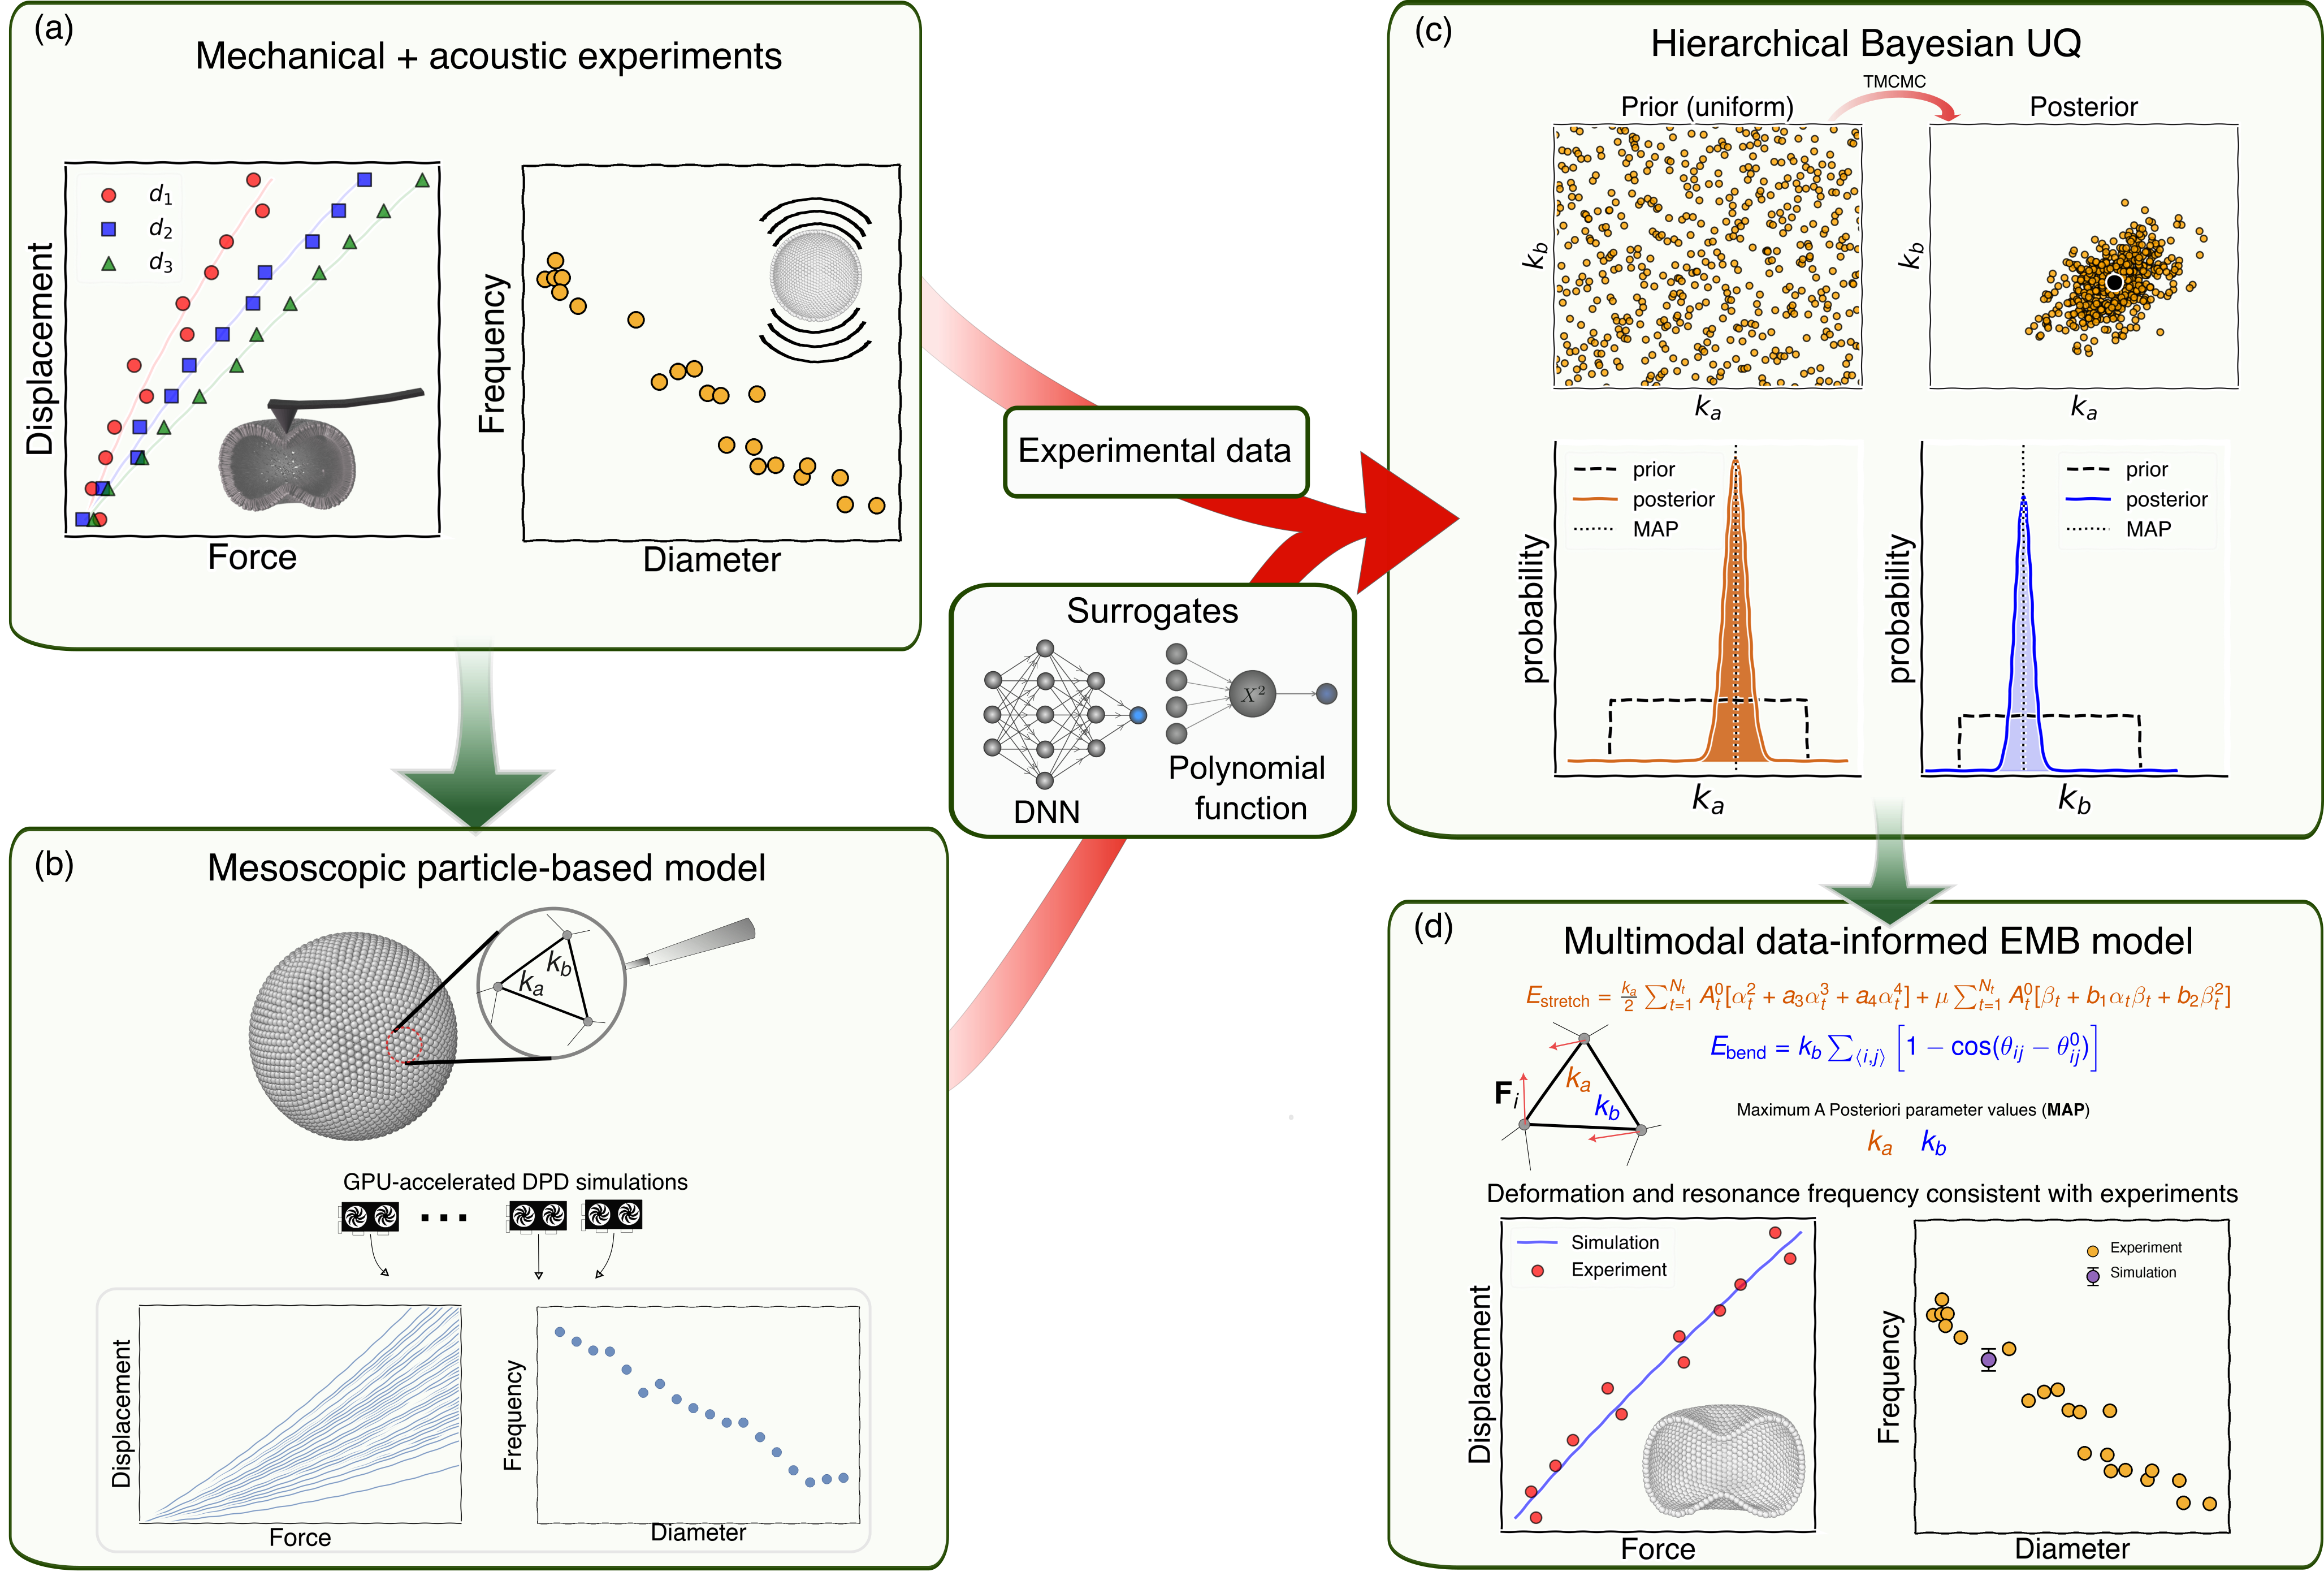
\includegraphics[width=1.0\linewidth]{Figure_1.png}
    \caption{Hierarchical Bayesian \textsc{uq}-driven multiscale workflow from experiments through large-scale simulations and surrogate models to a data-informed \textsc{emb} model. (a) Mechanical experiments, such as indentation or compression, provide force-displacement curves, while acoustic measurements provide frequency observations. (b) A mesoscopic model \cite{ntarakas2025dissipative}, solved using \textsc{gpu}-accelerated simulations, produces linear mechanical and acoustic-frequency responses through effective model parameters, generating an ensemble of responses across the parameter space. (c) A hierarchical Bayesian uncertainty quantification (\textsc{uq}) workflow, combined with \textsc{dnn} and polynomial surrogates (based on the ensemble of generated simulation data), enables efficient parameter inference from experimental data with quantified uncertainty. (d) The inferred posteriors, specifically the Maximum A Posteriori (\textsc{map}) values of the probability distributions, are then used to parameterize a calibrated \textsc{emb} model for subsequent large-scale simulations.}
    \label{fig:overview}
\end{figure}

\section{Methods}
\label{sec:methods}

\begin{figure}%[t]
\centering
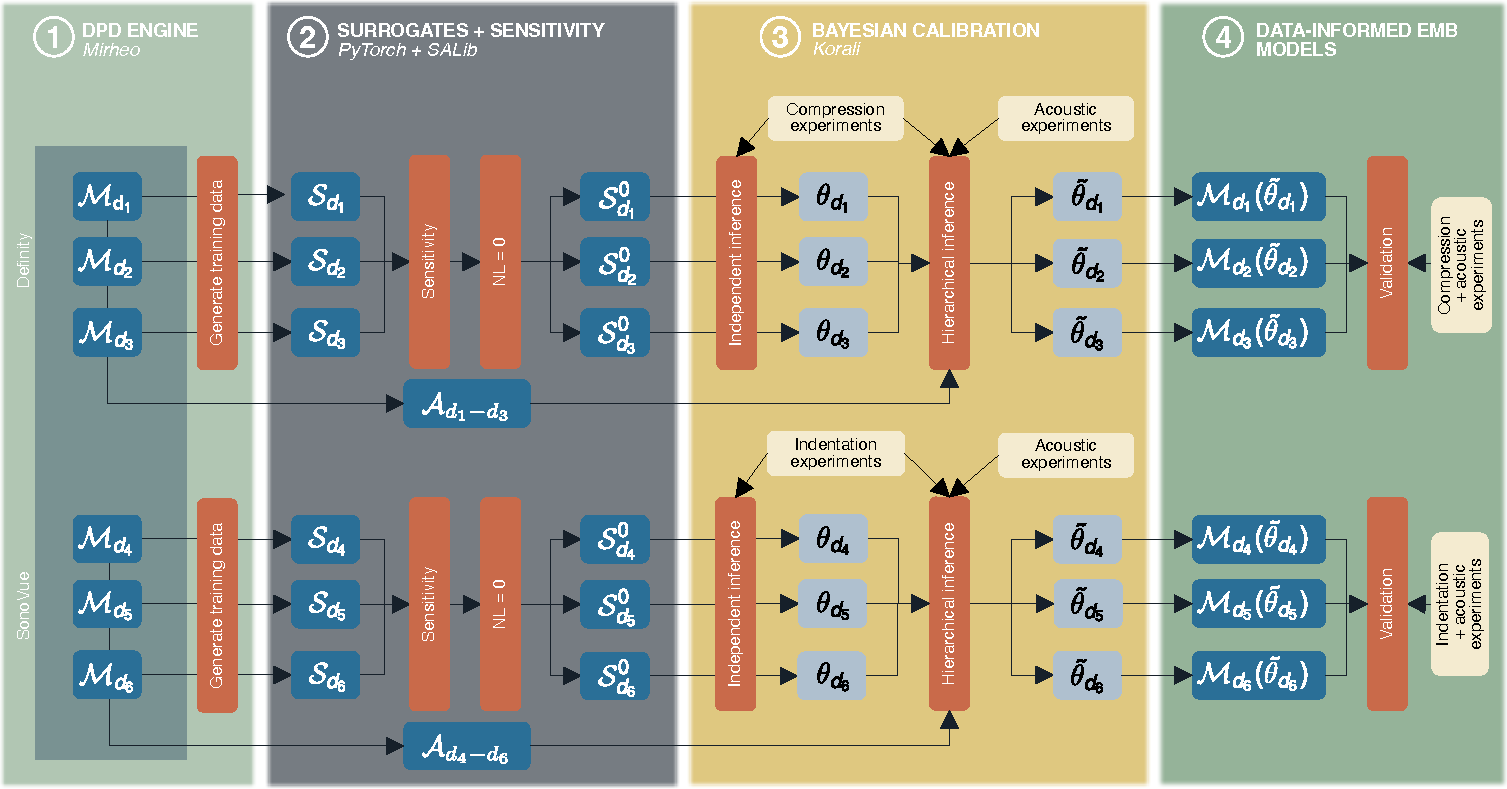
\includegraphics[width=1.\textwidth]{Figure_2.pdf}
\caption{Workflow diagram for the hierarchical Bayesian inference of data-informed \textsc{emb} models. $\mathcal{M}_{d_1,d_2,d_3}$ denote models of Definity bubbles, while $\mathcal{M}_{d_4,d_5,d_6}$ denote SonoVue bubbles. Throughout the workflow, the index $d_i$ labels the bubble diameter, with $(d_i)_{i=1,2,3,4,5,6}$ corresponding to $2.1$, $2.9$, $3.0$, $3.2$, $3.4$, and $5.8\,\mu$m, respectively. For each bubble $i$, the \textsc{dpd} model $\mathcal{M}_{d_i}$ generates mechanical and acoustic training data used to construct a \textsc{dnn} surrogate $\mathcal{S}_{d_i}$ and a polynomial surrogate $\mathcal{A}_{d_i}$, respectively. The mechanical surrogate is subsequently reduced to $\mathcal{S}_{d_i}^{0}$ through sensitivity analysis and suppression of nonlinear terms. Independent inference combines each mechanical surrogate with the corresponding compression (top row) or indentation (bottom row) experiment, yielding model parameters $\theta_{d_i}$. Hierarchical inference additionally includes the acoustic observations and yields regularized parameters $\tilde{\theta}_{d_i}$. The resulting calibrated model $\mathcal{M}_{d_i}(\tilde{\theta}_{d_i})$ is finally checked against the corresponding force spectroscopy data in the retained linear regime.}
\label{fig:workflow}
\end{figure}


%\textbf{\\\textsc{dpd} simulations}
\subsection{\textsc{dpd} simulations}
\label{sec:meth:dpd}

\noindent All mesoscale simulations were performed using \textsc{dpd}, a particle-based method well suited for modeling soft matter systems with explicit hydrodynamics~\citep{groot1997dissipative}. In \textsc{dpd}, each particle represents a coarse-grained cluster of molecules and evolves according to Newton's equations of motion. The total force acting on the particle $i$ is given by
\begin{equation}
\label{eq:forces_dpd}
\mathbf{F}_i = \sum_{j \neq i} \left(\mathbf{F}_{ij}^{\mathrm{C}} + \mathbf{F}_{ij}^{\mathrm{D}} + \mathbf{F}_{ij}^{\mathrm{R}} \right) + \mathbf{F}_i^{\mathrm{shell}},
\end{equation}
where $\mathbf{F}_{ij}^{\mathrm{C}}$, $\mathbf{F}_{ij}^{\mathrm{D}}$, and $\mathbf{F}_{ij}^{\mathrm{R}}$ are the conservative, dissipative, and random pairwise forces, respectively, and $\mathbf{F}_i^{\mathrm{shell}}$ denotes the elastic forces arising from the encapsulating microbubble shell.

The conservative force between particles $i$ and $j$ is defined as
\begin{equation}
\mathbf{F}_{ij}^{\mathrm{C}} =
\begin{cases}
a_{ij} \left(1 - r_{ij}/r_c \right) \hat{\mathbf{r}}_{ij}, & r_{ij} < r_c, \\
0, & r_{ij} \geq r_c,
\end{cases}
\end{equation}
where $r_{ij}$ is the interparticle distance, $\hat{\mathbf{r}}_{ij}$ the corresponding unit vector, and $r_c$ the cutoff radius. Dissipative and random forces are given by
\begin{align}
\mathbf{F}_{ij}^{\mathrm{D}} &= -\gamma \, \omega^{\mathrm{D}}(r_{ij}) 
\left(\hat{\mathbf{r}}_{ij} \cdot \mathbf{v}_{ij} \right) \hat{\mathbf{r}}_{ij}, \\
\label{eq:noise_dpd}
\mathbf{F}_{ij}^{\mathrm{R}} &= \sigma_\mathrm{DPD} \, \omega^{\mathrm{R}}(r_{ij}) \, \xi_{ij} \, \Delta t^{-1/2} \hat{\mathbf{r}}_{ij},
\end{align}
where $\mathbf{v}_{ij}$ is the relative velocity, $\xi_{ij}$ is a zero-mean unit-variance Gaussian random variable, and $\Delta t$ is the integration time step. The \textsc{dpd} fluid is simulated in reduced units following Ref.~\cite{ntarakas2025dissipative}. The cutoff radius is set to $r_c=1$ in simulation units and corresponds to $250~\mathrm{nm}$ in physical units, while the thermal energy is set to $k_B T=1$ and corresponds to room-temperature thermal energy. The water number density is set to $n_d=3$, which fixes the water-bead mass scale through the physical density of water. The dissipative coefficient is set to $\gamma=3.5$, and the random-force amplitude is fixed by the fluctuation--dissipation relation $ \sigma_\mathrm{DPD}^2=2\gamma k_B T$. The dissipative weight function is $\omega^{\mathrm{D}}(r)=(1-r/r_c)^2$ for $r<r_c$.

The encapsulating microbubble shell was modeled as a triangulated elastic surface immersed in a \textsc{dpd} solvent. Consistent with the fixed-thickness assumption used in the reference \textsc{afm} analyses \cite{buchner2012,morris2014mechanical}, the shell was treated as a thin membrane with a nominal thickness of $5~\mathrm{nm}$. Each vertex of the triangulation corresponds to a \textsc{dpd} particle, and elastic forces are obtained as derivatives of a discrete shell energy, inspired by recent data-driven red blood cell models \cite{walchli2020load,economides2021hierarchical,amoudruz2022simulations,amoudruz2023stress,amoudruz2024volume,amoudruz2025scalable}. Using expressions adopted from our previous work \cite{ntarakas2025dissipative}, the active shell energy in the present \textsc{emb} workflow is
\begin{equation}
E_{\mathrm{shell}} = E_{\mathrm{stretch}} + E_{\mathrm{bend}}.
\end{equation}
In-plane elastic deformations are described by
\begin{equation} \label{stretch_ene}
  E_{\mathrm{stretch}} = \frac{k_a}{2} \sum_{t=1}^{N_t} A_t^0[\alpha_t^2 + a_3 \alpha_t^3 + a_4 \alpha_t^4] + \mu \sum_{t=1}^{N_t} A_t^0[\beta_t + b_1 \alpha_t \beta_t + b_2 \beta_t^2],
\end{equation}
where $\alpha_t$ and $\beta_t$ are the area and shear strain invariants of the triangle $t$ and $A_t^0$ is the area of triangle $t$. This expression also includes nonlinear terms (coefficients $a_3, a_4, b_1$, $b_2$). Bending resistance is modeled via a dihedral-angle potential,
\begin{equation} \label{bend_ene}
  E_{\mathrm{bend}} = k_b\sum_{\langle i,j\rangle} \left[1-\cos(\theta_{ij}-\theta_{ij}^0)\right],
\end{equation}
with $\theta_{ij}$ and $\theta_{ij}^0$ the actual and spontaneous angles between two adjacent triangles \cite{bian2020bending}. We report the inferred in-plane stretching scale directly as $k_a$. We infer $k_b$ independently, as the stretching--bending relationship is model-dependent and less reliable for coated microbubbles. In contrast, we retain an isotropic in-plane law \cite{lim2002stomatocyte,Lim_H_W2009-hl}, since the data constrain only the dominant stiffness and do not support identification of a separate shear modulus. Accordingly, $\mu$ is not inferred independently and is related to $k_a$ through 
\begin{equation}
\mu = \frac{1-\nu}{1+\nu}\,k_a,
\end{equation}
which gives $\mu = k_a/3$ for the fixed Poisson ratio $\nu=0.5$ used throughout. The higher-order nonlinear elastic parameters $(b_1, b_2, a_3, a_4)$ are introduced to account for the large strains encountered in strongly deformed red blood cell morphologies, where linear elasticity fails, and these terms capture the strain-hardening response of the spectrin cytoskeleton, resulting in a marked increase in membrane stiffness and deformation energy at large strain \cite{lim2002stomatocyte,Lim_H_W2009-hl,bozic2012role}.

Both the surrounding liquid and the encapsulated gas were modeled explicitly using \textsc{dpd} particles. No-through boundary conditions at the membrane were enforced using a bounce-back mechanism~\citep{revenga1999boundary,fedosov2010multiscale}, while interfacial slip conditions were controlled by tuning the dissipative coupling parameters between shell, water, and gas particles. The treatment of the gas phase, including pressure compensation and ideal-gas behavior, follows exactly the methodology described in Ref.~\cite{ntarakas2025dissipative}. All simulations were performed using the \textsc{gpu}-accelerated \textsc{dpd} framework \textsc{mirheo} \cite{alexeev2020mirheo}. To ensure computational feasibility while preserving the relevant elastic physics, all elastic moduli of the shell were uniformly downscaled by a factor $f_{scale} = 0.0074$ \cite{ntarakas2025dissipative}, which preserves the F\"oppl--von K\'arm\'an number \cite{paulose2012fluctuating} and thus the equilibrium and deformation behavior of the shell. Physical forces were recovered by rescaling during post-processing \cite{ntarakas2025dissipative}. The mechanical response of the shell was characterized by extracting force–displacement relations through two distinct simulation protocols: indentation and compression.


Indentation simulations mimic \textsc{afm} indentation experiments by applying equal and opposite external forces to sets of shell vertices located near the top and bottom poles of the microbubble, see Fig.~\ref{fig:dpd_scheme}(a). The equatorial vertices were constrained in the axial direction to suppress rigid-body motion. For each applied force level, the system was equilibrated quasi-statically, and the resulting axial displacement of the shell was recorded. Force--displacement curves were obtained by prescribing the force and measuring the displacement. Parallel-plate compression simulations were implemented using two rigid plates represented by a dense collection of frozen particles, see Fig.~\ref{fig:dpd_scheme}(b). The plates were pinned to move only along the axial direction and displaced quasi-statically toward the microbubble. After equilibration, the reaction force exerted by the shell on the plates was recorded. In this case, force--displacement curves were obtained by prescribing displacement and measuring the resulting reaction force. More information about the reference experimental setups can be found in Section S2 in the supplementary material.

Acoustic response data were generated by isotropically compressing each equilibrated bubble by 5\%, releasing it, and recording the relaxation of the root-mean-square bubble radius. The relaxation was fitted with a damped sinusoid. Writing $\omega_d$ for the fitted damped angular frequency and $\lambda$ for the decay rate, we define the resonance frequency as $f_{\mathrm{res}}=(\omega_d^2-\lambda^2)^{1/2}/(2\pi)$ (Section S5 in the supplementary material). Although the breathing frequency can be extracted using the principal-component analysis (PCA) employed in Ref.~\cite{ntarakas2025dissipative}, we selected the relaxation protocol because its shorter simulation time reduces the cost of generating the training data for the polynomial surrogates. We nonetheless confirmed that our procedure agrees with the PCA estimates, with a mean absolute relative difference of 3.2\% and a maximum of 5.9\% (Table S7 in the supplementary material). In the PCA protocol, we identify the breathing mode as the PCA eigenvector having the largest absolute overlap with uniform radial motion, following the radial mode-projection criterion of Ref.~\cite{papez2023subthz}.

\begin{figure}
    \centering
    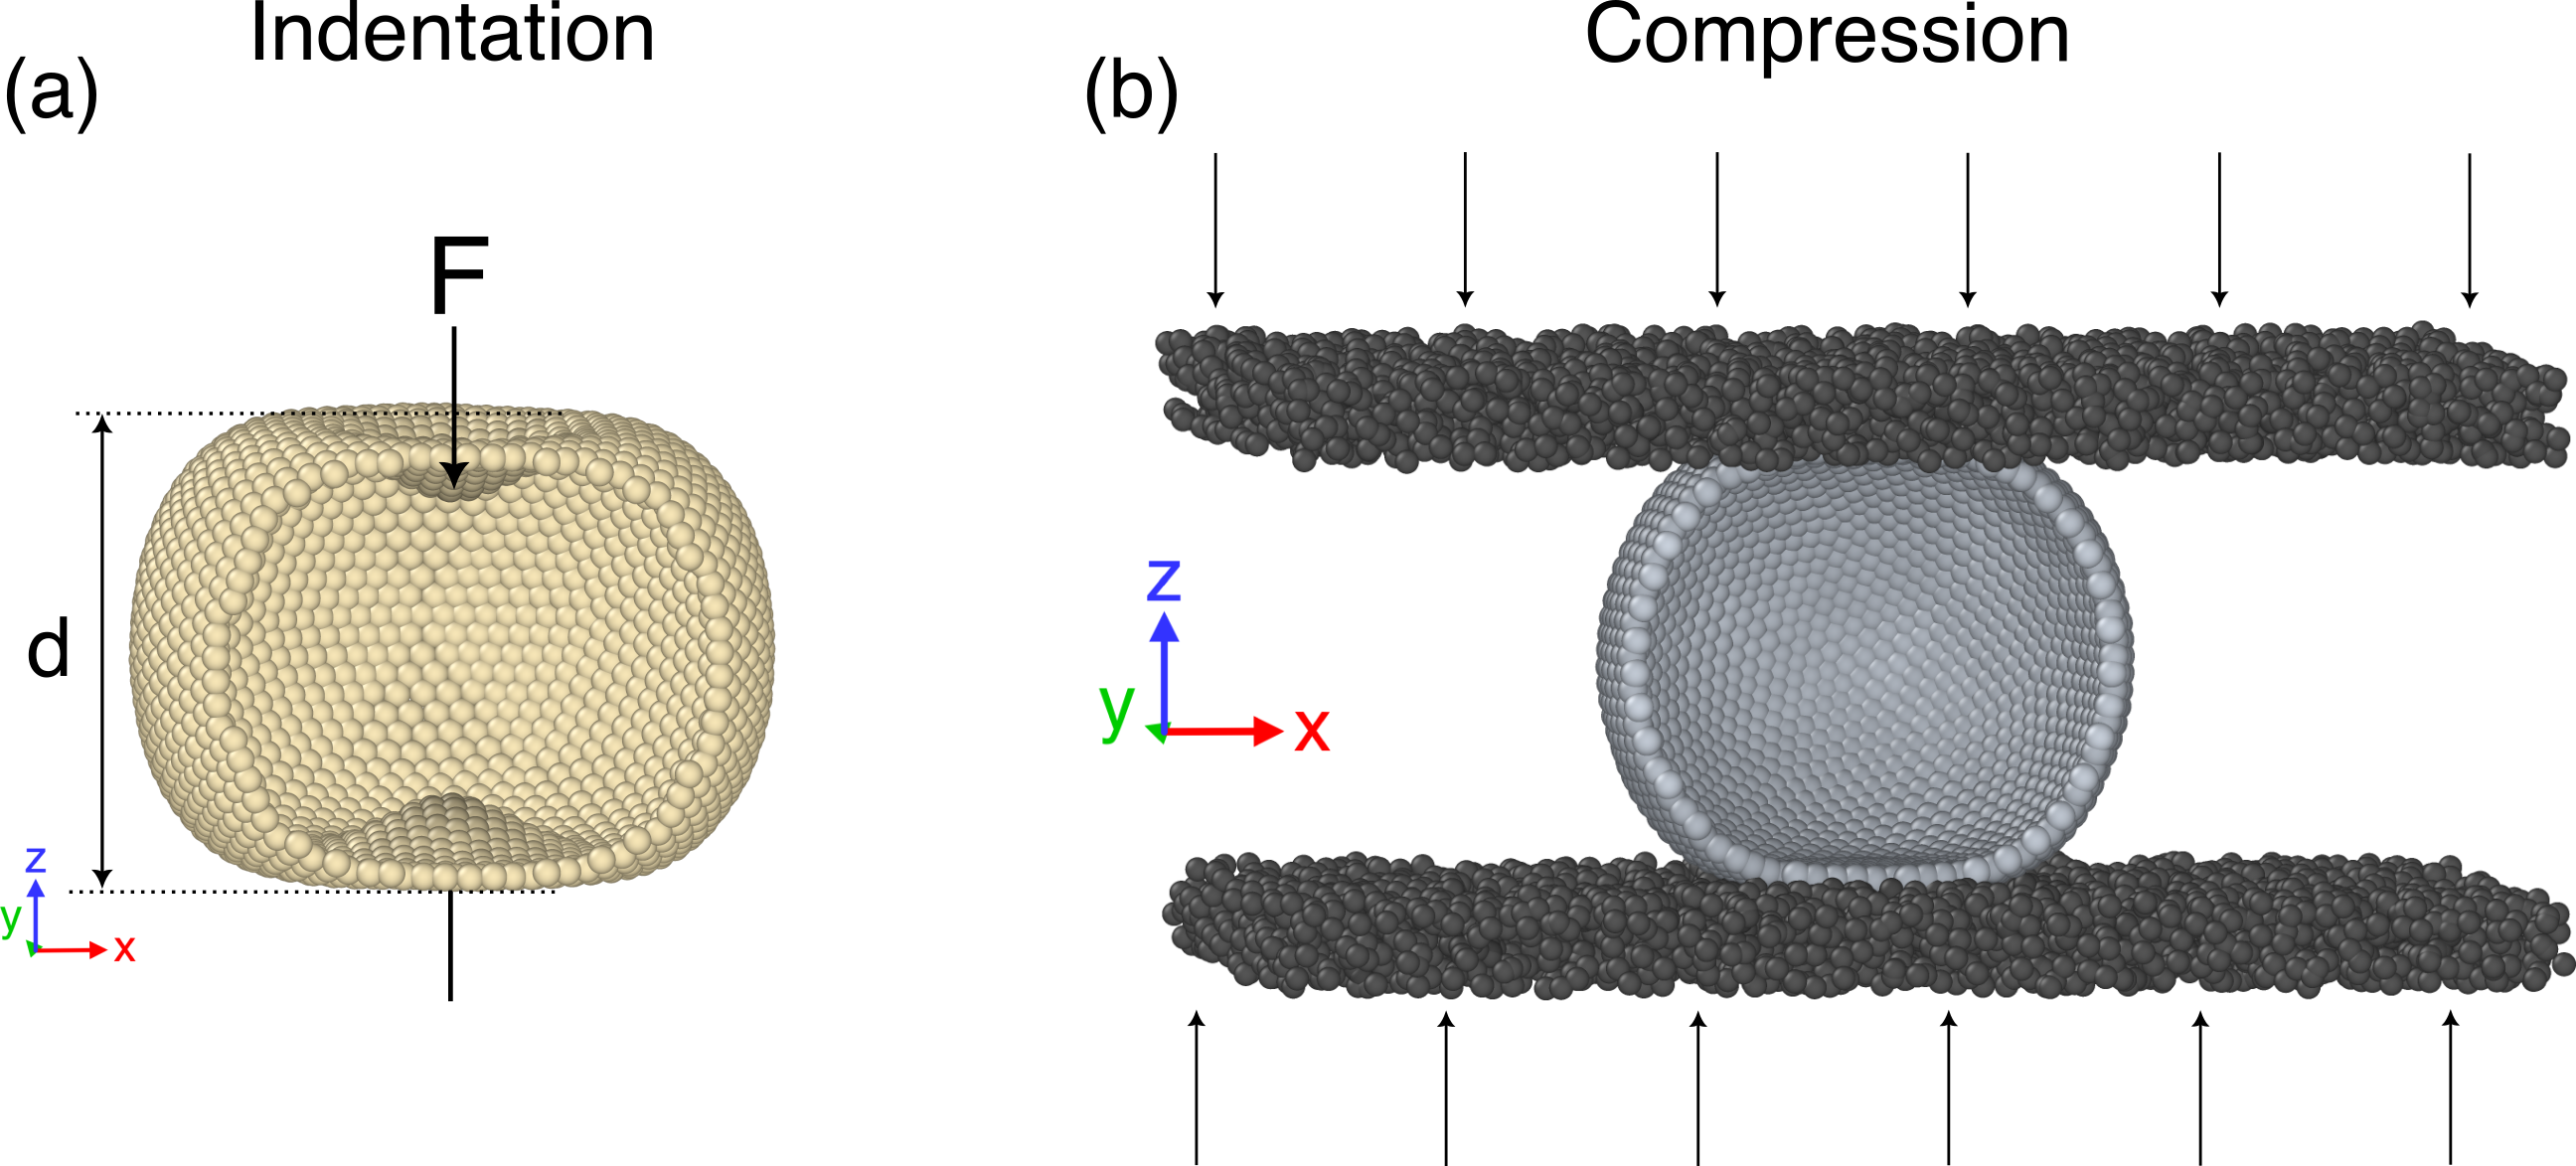
\includegraphics[width=1.0\linewidth]{Figure_3.png}
    \caption{A schematic representation of the \textsc{dpd} simulations implemented in this work. (a) Indentation simulations are performed on a SonoVue microbubble (gold) by applying a pair of equal and opposite forces to a small fraction of vertices at the top and bottom of a microbubble. (b) The plate compression is implemented by displacing a set of frozen \textsc{dpd} particles, representing a large cantilever used in the compression of a Definity microbubble (ink).}
    \label{fig:dpd_scheme}
\end{figure}


%\textbf{\\Deep neural network (\textsc{dnn}) surrogates}
\subsection{Surrogates}
\label{sec:methods_surrogates}

  \noindent Direct evaluation of the mechanical and acoustic responses of an \textsc{emb} with \textsc{dpd} simulations is computationally expensive, making it impractical within large-population Bayesian inference runs. Each \textsc{dpd} model $\mathcal{M}_{d_i}$ therefore generates mechanical and acoustic simulation data used to construct a \textsc{dnn} surrogate $\mathcal{S}_{d_i}$ for force spectroscopy and a polynomial surrogate $\mathcal{A}_{d_i}$ for resonance frequency, respectively. The surrogates replaced the corresponding \textsc{dpd} models during inference and uncertainty propagation (see Fig.~\ref{fig:workflow} for details). In all cases, the surrogate was trained to approximate \textsc{dpd} outputs for a fixed \textsc{emb} model and a fixed \textsc{emb} diameter. Six \textsc{dnn} surrogates were constructed, one for each of the three mechanically calibrated diameters within both \textsc{emb} models. Compression surrogates predicted force at prescribed displacement, whereas indentation surrogates predicted displacement at prescribed force. All surrogate inputs were written directly in terms of $(k_a,k_b,\ldots)$, consistent with the parameterization used throughout the Results section. We trained a separate surrogate per diameter and retained the best-performing model for each diameter for use in the inference pipeline. Implementation details, including how the best model was selected, are summarized in Section S5 in the supplementary
  material.

For the acoustic response, we fitted one polynomial surrogate per simulated diameter using frequencies extracted from \textsc{dpd} relaxation simulations. The resonance frequency $f_{\mathrm{res}}$ is insensitive to $k_b$: varying $k_b$ across its admissible range changed the frequency by less than 0.5\% in our numerical tests. This is expected because uniform radial motion preserves the shell angles by symmetry, so the bending term does not contribute to the restoring force at leading order and the frequency is governed primarily by $k_a$. Small-amplitude radial oscillations can be formulated as the generalized eigenvalue problem $\mathbf{K}(k_a)\mathbf{u}=\omega^2\mathbf{M}\mathbf{u}$, making the squared frequency the natural quantity to approximate. We therefore define
\begin{equation}
f_{\mathrm{res},d_i}^2(k_a)=a_{0,d_i}+a_{1,d_i}k_a+a_{2,d_i}k_a^2,
\end{equation}
and the surrogate $\mathcal{A}_{d_i}(k_a)$ predicts the value of $f_{\mathrm{res}}$ given by this fitted relation. The quadratic is the lowest-order form that captures the curvature observed in the simulated data. Each polynomial surrogate is evaluated only within its simulated $k_a$ range. Frequency extraction, polynomial-surrogate definition, simulated $k_a$ ranges, and validation are detailed in Section S5 in the supplementary material.
  
%\textbf{\\Bayesian inference framework}
\subsection{Bayesian inference framework}
\label{sec:meth:bayes}

\noindent We calibrated the \textsc{emb} force field parameters with \textsc{tmcmc}~\cite{ching2007transitional} as implemented in \textsc{korali}~\cite{martin2022korali}. The full and reduced workflows share the same inferential structure; unless otherwise stated, the reported results correspond to the reduced model, in which $(b_1,b_2,a_3,a_4) = (0,0,0,0)$, while the full model is used only for a spectroscopy consistency check. For each diameter-specific reference curve $i$, the reference dataset is a set of $N_i$ paired observations $\mathcal{D}_i = \{(x_{ij}, y_{ij})\}_{j=1}^{N_i}$. For compression (resp. indentation) experiments, $x_{ij}$ denotes displacement (resp. force) and $y_{ij}$ denotes force (resp. displacement). The diameter-specific parameter vector is $\Theta_{d_i} = \bigl(k_a, k_b, b_1, b_2, a_3, a_4, d_0\bigr)_{d_i}$, where $(k_a,k_b,b_1,b_2,a_3,a_4)$ are the constitutive parameters and $d_0$ is a calibration offset. It is introduced to absorb uncertainty in the experimental bubble-cantilever contact position, since the \textsc{dpd} setup does not explicitly model the details of the cantilever adhesion to the bubble during initial contact. The observation-noise amplitude is denoted separately by $\sigma_{d_i}$ and is shared across all points of a given curve. For clarity, we omit the explicit diameter dependence in $\Theta_{d_i}$ and $\sigma_{d_i}$ in this section and write $\Theta_i$ and $\sigma_{i}$ instead. The calculations are presented in terms of the full parameter set $\Theta_i$ but apply equally to the reduced parameter set  $\theta_i$. 

We use a Gaussian likelihood with multiplicative noise: the per-point standard deviation $s_{ij}(\Theta_{i})$ is proportional to the model prediction $s_{ij}(\Theta_{i}) = \sigma_{i}\,\hat{y}_{ij}$,
where $\sigma_i$ is the diameter-specific observation-noise amplitude. This yields
\begin{equation}
P(\mathcal{D}_i \mid \Theta_{i}, \sigma_i) = \prod_{j=1}^{N_i} \mathcal{N}\!\left(y_{ij} \,\middle|\, \hat{y}_{ij},\, s_{ij}(\Theta_{i})^2\right).
\end{equation}
In the independent inference step, each diameter $d_i$ of each \textsc{emb} model is treated independently. We assign independent uniform priors to all components of $\Theta_{i}$ and sample the diameter-specific posterior,
\begin{equation}
P(\Theta_{i} \mid \mathcal{D}_i)\ \propto\ P(\mathcal{D}_i \mid \Theta_{i})\,P(\Theta_{i}).
\end{equation}
The prior and hyperprior ranges for the spectroscopy-only full model and the acoustically conditioned reduced model are summarized in Table S4 in the supplementary material. The reduced-model workflow
  uses the same mechanical likelihood, data, and phase structure, but fixed $(b_1,b_2,a_3,a_4)=(0,0,0,0)$ and infers only $(k_a,k_b,d_0,\sigma)$. These
  reduced independent inference runs provide the baseline single-diameter posteriors used in Results before information is pooled hierarchically across
  diameters. Hierarchical regularization was performed separately within each bubble type; no sharing was performed across types. The reduced workflow
  additionally conditions the hierarchical stage on acoustic measurements evaluated using the acoustic surrogates described above. To
  pool information across diameters, we introduce hyperparameters for each Definity and
  SonoVue \textsc{emb} model
  \begin{equation}
  \psi = \{(m_k,\tau_k)\}_{k\in\mathcal{K}},\qquad
  k\in\mathcal{K}=\{k_a,k_b,b_1,b_2,a_3,a_4,d_0\}
  \end{equation}
  with Gaussian conditional priors for the hierarchical parameters $\Theta_{i,k}\mid\psi \sim \mathcal{N}(m_k,\tau_k^2)$, and uniform hyperpriors on
  $(m_k,\tau_k)_k$. For each parameter $k\in\mathcal{K}$, the conditional prior was truncated to the corresponding admissible range reported in Table
  S4 in the supplementary material. The mechanical and acoustic observation-noise amplitudes are inferred independently for each dataset and are not
  hierarchically pooled. The hyperparameter posterior for each \textsc{emb} model is conditioned on both the mechanical datasets $\mathcal{D}_i$ and the acoustic observations $f_j$,
  \begin{equation}
  P(\psi \mid \{\mathcal{D}_i\},\{f_j\})
  \propto
  P(\psi)
  \prod_i P(\mathcal{D}_i\mid\psi)
  \prod_j P(f_j\mid\psi).
  \end{equation}
  Each mechanical and acoustic dataset contributes a separate marginal likelihood under the same \textsc{emb} hierarchy, with its own parameter vector and observation-noise amplitude. \textsc{tmcmc} is then used to sample the hyperparameter posterior implied by the hierarchical model.
  Operationally, this phase learns the priors used by the final hierarchical posteriors; it is therefore an intermediate hierarchical-learning step rather than a standalone result. Hierarchical pooling produces the final diameter-specific posteriors reported in this work. This yields, for each
  bubble $i$, a posterior conditioned on hierarchical priors inferred jointly from the separate mechanical and acoustic datasets of the same
  \textsc{emb} model,
  \begin{equation}
  P(\Theta_i,\sigma_i \mid \mathcal{D}_i, \psi) \ \propto\ P(\mathcal{D}_i \mid \Theta_i,\sigma_i )\,P(\Theta_i \mid \psi)\,P(\sigma_i), \qquad \psi
  \sim P(\psi \mid \{\mathcal{D}_i\},\{f_j\})
  \end{equation}
  where $i$ runs over the diameters of each \textsc{emb} model. The \textsc{map} estimate was approximated by the posterior sample with the largest
  log-posterior value.

%\textbf{\\Uncertainty Propagation}
\subsection{Uncertainty Propagation}
\label{sec:meth:propagation}

\noindent Once the posterior distribution has been estimated, we propagate this uncertainty to the predicted response through the corresponding mechanical or acoustic surrogate. For any output quantity of interest $y$, the posterior predictive distribution is
\begin{equation}
P\!\left(y \mid \mathcal{D}_i\right)
=
\int
P\!\left(y \mid \Theta_i, \sigma_i\right)\,
P\!\left(\Theta_i, \sigma_i \mid \mathcal{D}_i\right)\,
d\Theta_i\, d\sigma_i
\;\approx\;
\frac{1}{N}\sum_{k=1}^{N}
P\!\left(y \mid \Theta_i^{(k)}, \sigma_i^{(k)}\right),
\end{equation}
where $(\Theta_i^{(k)},\sigma_i^{(k)}) \sim P(\Theta_i,\sigma_i \mid \mathcal{D}_i)$ are samples from the posterior retained for propagation. Here, $P(\Theta_i,\sigma_i \mid \mathcal{D}_i)$ denotes the posterior used for propagation, namely the final hierarchically regularized diameter-specific posterior in the hierarchical stage. In our case, $y$ is the response evaluated along the experimental grid, namely force at fixed displacement for compression and displacement at fixed force for indentation. For each posterior sample, the surrogate provides a mean response, while the observation model assigns a Gaussian uncertainty with standard deviation $\sigma_i^{(k)} \hat{y}^{(k)}$ proportional to that prediction. The posterior predictive distribution at each grid point is therefore represented as a Gaussian mixture induced by the ensemble of posterior samples. In practice, we drew $N=5{,}000$ posterior samples and evaluated the corresponding predictive distribution pointwise along the experimental reference grid. Posterior medians and central predictive intervals, including the posterior median and the pointwise 90\% posterior predictive
interval reported in this paper, were then obtained by numerical inversion of the corresponding cumulative distribution function (\textsc{cdf}) at each grid point. These posterior predictive bands are therefore fully consistent with the same heteroscedastic Gaussian likelihood used during inference, and were used to assess coverage against the experimental observations. Acoustic predictive intervals were obtained analogously by propagating posterior samples through the corresponding acoustic surrogates and combining the predictions with the inferred acoustic observation noise.

%\textbf{\\Continuous ranked probability score (\textsc{crps})}
\subsection{Continuous ranked probability score (\textsc{crps})}
\label{sec:meth:crps}

\noindent To complement interval inclusion with one proper scoring rule, we also report the \textsc{crps} for the six datasets discussed in Results~\citep{gneiting2007strictly,gneiting2007probabilistic,hersbach2000decomposition}. For a retained experimental point $j$ with observed response $y_j$ and pointwise posterior predictive \textsc{cdf} $F_j$, the score is
\begin{equation}
\mathrm{CRPS}(F_j,y_j)=\int_{-\infty}^{\infty}\left(F_j(z)-\mathbf{1}\{z\ge y_j\}\right)^2\,dz \, ,
\end{equation}
with lower values indicating better probabilistic agreement. In the present workflow, $F_j$ is the pointwise Gaussian mixture induced by the propagated posterior samples and the heteroscedastic noise model above. The posterior-predictive bands shown in the figures are obtained from pointwise quantiles of this mixture distribution, computed by numerical inversion of the corresponding \textsc{cdf}. For \textsc{crps}, we approximate the same pointwise posterior predictive distribution by Monte Carlo: for each retained posterior sample, we draw one response from its associated Gaussian component, compute the empirical ensemble \textsc{crps} at point $j$, and then average over the retained points of each curve to obtain the reported mean \textsc{crps}. The reported values are further averaged over five independent Monte Carlo replicates. We use \textsc{crps} because, unlike coverage alone, it rewards both calibration and sharpness under the same posterior predictive distribution.

%\textbf{\\Transitional Markov Chain Monte Carlo (\textsc{tmcmc})}
\subsection{Transitional Markov Chain Monte Carlo (\textsc{tmcmc})}
\label{sec:meth:tmcmc}

\noindent Posterior sampling was performed with \textsc{tmcmc} as implemented in \textsc{korali}~\citep{martin2022korali} and executed in parallel with \textsc{mpi}. \textsc{tmcmc} builds a sequence of intermediate tempered distributions connecting prior and posterior, which improves robustness in parameter spaces that are broad, correlated, or otherwise difficult to explore directly. The numerical \textsc{tmcmc} settings used in production are reported in Section S6 in the supplementary material.



%\textbf{\\Computational Implementation}
\subsection{Computational Implementation}
\label{sec:meth:implementation}

\noindent All workflows were executed on a high-performance computing environment consisting of multi-core \textsc{cpu} nodes and \textsc{cuda}-capable \textsc{gpu} nodes. Direct \textsc{dpd} simulations were performed with \textsc{mirheo}, while Bayesian inference used \textsc{korali} with \textsc{mpi} parallelization. The \textsc{dnn} and polynomial surrogates were constructed and evaluated in Python using PyTorch and standard scientific Python libraries, with all workflow settings provided through \textsc{yaml} configuration files. More computational details can be found in Section S1 in the supplementary material.


\section{Results and Discussion}
\label{sec:results}

Results are reported for two \textsc{emb} models of commercial agents with different lipid shells (Definity and SonoVue) and three bubble diameters per \textsc{emb} model. Definity models are calibrated using experimental data from \textsc{afm} compression, whereas SonoVue models are calibrated with data from \textsc{afm} indentation. The inference conditions on one reprocessed published curve per diameter (see Fig. S1 in the supplementary material); the exact source references and retained point counts are summarized in Table S3 in the supplementary material. The published force spectroscopy curves contain an initial linear loading regime followed by a nonlinear response at larger deformation, but the likelihood uses only the retained points in the linear regime listed in Table S3. We first use the full membrane force field only to establish the sensitivity structure of the inverse problem and then, from the sensitivity section onward, carry a reduced model with membrane parameters $(k_a,k_b)$ through the main-text inference workflow, treating $d_0$ and $\sigma$ separately as calibration and noise parameters. The full model is rerun only against the same retained force spectroscopy data in the sanity-check section. 

\subsection{{\textsc{dpd}} force field and \textsc{dnn} surrogate validation}
\label{sec:res:dpd_surrogate}

\begin{figure}%[t]
\centering
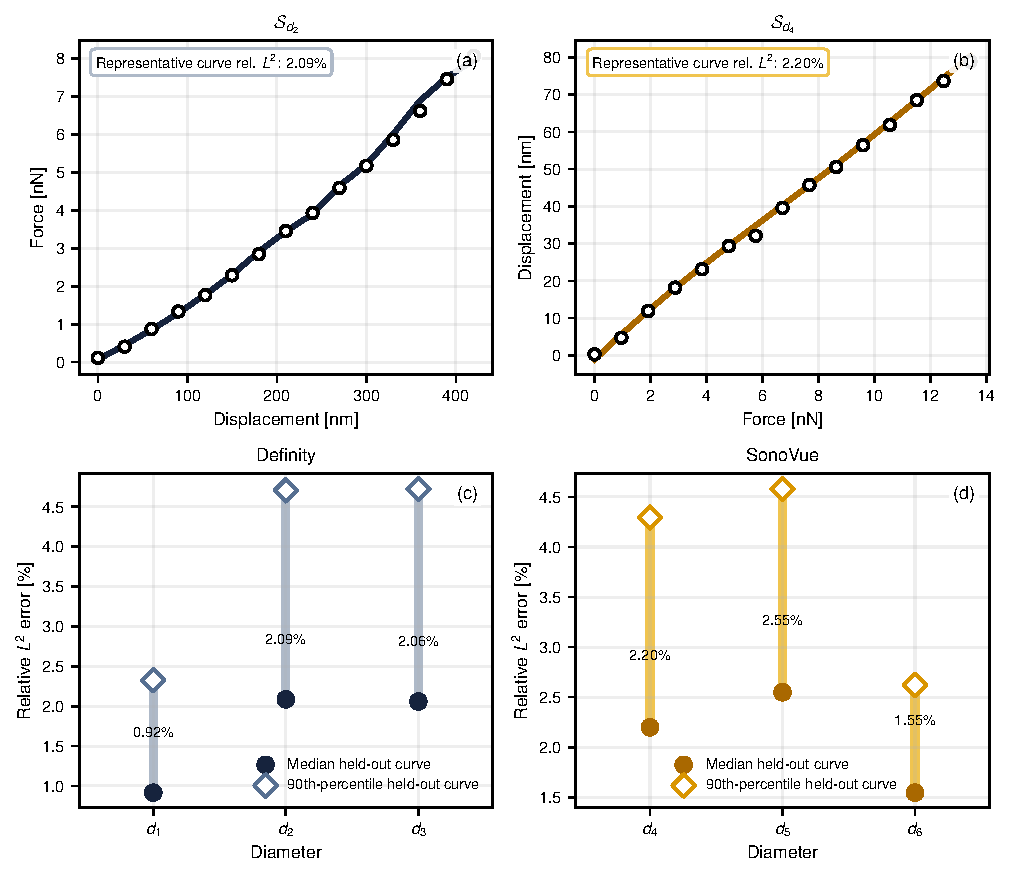
\includegraphics[width=0.98\linewidth]{Figure_4.pdf}
\caption{Grouped-holdout \textsc{dnn} surrogate validation. Panels (a–b) compare held-out \textsc{dpd} curves with the corresponding \textsc{dnn} predictions for representative $\mathcal{S}_{d_2}$ and $\mathcal{S}_{d_4}$ surrogates for Definity (ink) and SonoVue (gold), respectively; open circles denote held-out \textsc{dpd} points and solid lines denote surrogate predictions. Panels (c–d) summarize, for each \textsc{emb} model, the median and $90^{th}$-percentile held-out-curve relative $L^2$ errors from the grouped parameter-set holdout audit; filled circles and open diamonds denote these statistics, respectively.}
\label{fig:surrogate_validation_curves}
\end{figure}

We consider six \textsc{dpd} models $(\mathcal{M}_{d_i})_{i \in [1,6]}$, which share the same physical formulation and parameterization~\citep{ntarakas2025dissipative}, but correspond to different experimental conditions (see Fig.~\ref{fig:workflow}, block \textcircled{1}). Models $\mathcal{M}_{d_1}, \mathcal{M}_{d_2}, \mathcal{M}_{d_3}$ describe Definity bubbles~\cite{lindner2002microvascular,datta2008ultrasound,baseri2010multi} (compression experiments) for fixed diameters ($d_1, d_2, d_3$) respectively, while $\mathcal{M}_{d_4}, \mathcal{M}_{d_5}, \mathcal{M}_{d_6}$ describe SonoVue bubbles~\cite{schneider1999sonovue,demene2021transcranial,tu2009estimating,guo2013investigation,de2007compression} (indentation experiments) for fixed diameters ($d_4, d_5, d_6$) respectively. Throughout, $d_i$ denotes the bubble diameter. The six diameters, in $\mu\mathrm{m}$, are $d_1=2.1$, $d_2=2.9$, $d_3=3.0$, $d_4=3.2$, $d_5=3.4$, and $d_6=5.8$. We simulate the \textsc{dpd} models using the high-performance \textsc{mirheo} software package \cite{alexeev2020mirheo}. In the compression experiment with Definity, the \textsc{dpd} simulation returns the reaction force as a function of imposed displacement through an explicit plate-contact geometry. In the indentation experiment with SonoVue, it returns the bubble diameter change as a function of applied force under the prescribed loading protocol. These \textsc{dpd} outputs are therefore directly comparable to the corresponding experimental measurements. The membrane force field of each model $\mathcal{M}_{d_i}$ is parameterized by a stretching stiffness $k_a$, a bending modulus $k_b$, nonlinear elastic coefficients $(b_1, b_2, a_3, a_4)$, and a displacement offset $d_0$ used to align the curves. These parameters are collected in the associated vector $\Theta_{d_i} = (k_a, k_b, b_1, b_2, a_3, a_4, d_0)_{d_i}$ while the observation-noise amplitude $\sigma_{d_i}$ is treated separately as a diameter-specific parameter. Full details of the \textsc{dpd} setup and parameter definitions are provided in the Methods section.

To enable Bayesian inference at scale, we train \textsc{dnn} surrogates to predict the output of the \textsc{dpd} models on thousands of simulated curves. Each \textsc{dpd} model~$\mathcal{M}_{d_i}$ is subsequently replaced by its surrogate counterpart~$\mathcal{S}_{d_i}$ (see Fig.~\ref{fig:workflow}, block~\textcircled{2}) during inference, enabling efficient Bayesian calibration. Surrogate selection is performed via an architecture sweep, retaining the \textsc{dnn} with the lowest grouped-holdout median relative $L^2$ error. The grouped holdout excludes entire simulated curves from training and therefore evaluates generalization to unseen parameter sets~\cite{ma2020eating}. In this validation, the median relative $L^2$ error over the full loading branch remains low: less than 2.1\% for Definity surrogates and less than 2.6\% for SonoVue surrogates (see Table S2 in the supplementary material). Fig.~\ref{fig:surrogate_validation_curves} combines representative grouped-holdout curves in real units with a compact across-diameter summary based on the median and 90th-percentile held-out-curve relative $L^2$ errors, showing low surrogate error for most held-out simulated curves. Representative held-out grouped-validation curves are collected in Fig. S2 in the supplementary material. Combined with their orders-of-magnitude speedup over direct simulation, these surrogate errors are low enough to make the subsequent \textsc{tmcmc}-based calibration computationally tractable, see Methods section.

\subsection{Sensitivity analysis motivates a reduced membrane model}
\label{sec:res:sensitivity}

\begin{figure}%[htb!]%[t]
\centering
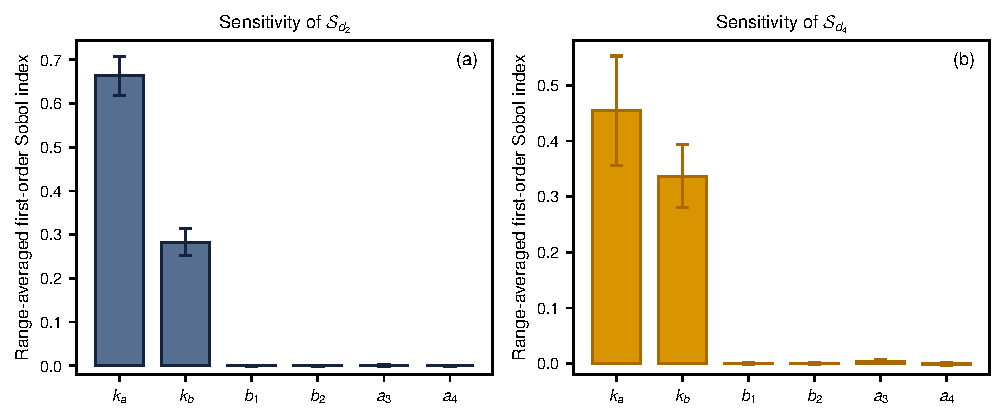
\includegraphics[width=0.98\linewidth]{Figure_5.pdf}
\caption{Range-averaged first-order Sobol sensitivity indices for representative diameters of each \textsc{emb} model. The bars report the loading-range-averaged first-order index for each material parameter for (a) Definity ($\mathcal{S}_{d_2}$, ink) and (b) SonoVue ($\mathcal{S}_{d_4}$, gold); error bars denote the corresponding averaged Sobol confidence estimates. Only the material parameters are shown.}
\label{fig:sensitivity}
\end{figure}

To determine which force field parameters can be constrained by force spectroscopy data, we quantify the global sensitivities of the \textsc{dnn} surrogates over the experimentally explored range using first-order Sobol indices \cite{herman2017salib}. Details of the sensitivity analysis are given in Section S7 in the supplementary material. The resulting hierarchy is clear: the response is governed primarily by the stretching stiffness $k_a$ and the bending modulus $k_b$, while the nonlinear coefficients $(b_1,b_2,a_3,a_4)$ contribute only weakly within the loading regime probed here. Fig.~\ref{fig:sensitivity} reports range-averaged first-order indices for representative surrogates $\mathcal{S}_{d_2}$ and $\mathcal{S}_{d_4}$. For $\mathcal{S}_{d_2}$, the indices assign approximately $66\%$ of the variance to $k_a$ and $28\%$ to $k_b$. For $\mathcal{S}_{d_4}$, the same averaged analysis assigns approximately $45\%$ to $k_a$ and $33\%$ to $k_b$. In both cases, the nonlinear terms remain negligible compared to the two elastic parameters, with bar heights clustered near zero within their confidence intervals. These representative panels are shown because they reflect the same dominant $k_a/k_b$ sensitivity structure observed separately for Definity and SonoVue surrogates. 

These sensitivity results indicate which parameters the present data are likely to constrain: in this deformation regime, the data primarily inform $(k_a,k_b)$, while the nonlinear terms are expected to remain weakly constrained. This motivates the concrete modeling decision adopted in the remainder of this study: after this section, the inference uses a reduced membrane force field with $(k_a,k_b)$ as the shell-mechanics parameters, while $d_0$ and $\sigma$ are retained separately as calibration and noise parameters. In practice, for each bubble $i$, we use the surrogates $\mathcal{S}_{d_i}^0$ obtained by setting the $\mathcal{S}_{d_i}$ nonlinear parameters $(b_1, b_2, a_3, a_4)$ to zero and we use the notation $\theta_{d_i}$ to refer to the associated reduced set of parameters (see Fig.~\ref{fig:workflow}, block \textcircled{2}): $\theta_{d_i} = (k_a, k_b, d_0)_{d_i}$. We return to the full models only in the Results section as a safety check on this reduction. 

\subsection{Hierarchical Bayesian inference of the reduced model}
\label{sec:res:phase1}
To establish a results baseline, we first perform independent Bayesian calibrations for each diameter using only the reduced models and force spectroscopy data in the retained linear regime (see Fig.~\ref{fig:workflow}, block \textcircled{3}). For each bubble $i$ (compression experiment using Definity: 2.1, 2.9, and 3.0~$\mu$m; indentation experiment using SonoVue: 3.2, 3.4, and 5.8~$\mu$m), we run a separate \textsc{tmcmc} inference using the \textsc{korali} software framework \cite{martin2022korali} and the corresponding \textsc{dnn} surrogate as the forward model, where $d_0$ is an auxiliary curve-alignment parameter and $\sigma$ controls the (relative) observation noise model (Methods). These spectroscopy-only calibrations, shown as grey areas in Fig.~\ref{fig:phase1_vs_phase3b_reduced_summary}, identify extended compatible regions in the $(k_a,k_b)$ plane rather than a unique parameter pair. This ridge-like degeneracy is consistent with the continuum analysis in Ref.~\cite{lytra2020modeling}, where the Reissner regime predicts the slope of the response curve to be proportional to $\sqrt{k_a k_b}$. 

The approach adopted by these authors to solve the degeneracy is to use the nonlinear part of the force--displacement curve to separate shell parameters.
However, this route is not usable in the present \textsc{dpd} model because the \textsc{dpd} pressure is chosen to be lower than the real values to ensure stable simulations and therefore does not reproduce the experimental internal/external pressure state of real bubbles. In particular, the internal gas pressure is low and is not increased during volume compression as in a physical bubble. Consequently, the nonlinear stiffening described in Ref.~\cite{lytra2020modeling} as a result of the response of the shell to gas compression is not captured at comparable deformations. Instead, the present \textsc{dpd} \textsc{emb} models leave the intended elastic regime and show nonphysical rupture or interpenetration. We therefore use acoustic frequency measurements as an independent constraint on $k_a$. The frequency observables are evaluated using the acoustic surrogates described in Methods. Before including the acoustic data in the hierarchy, we assessed the underlying polynomial surrogates by leave-one-out validation at every diameter associated with a retained acoustic measurement.

\begin{figure}%[!htb]%[t]
\centering
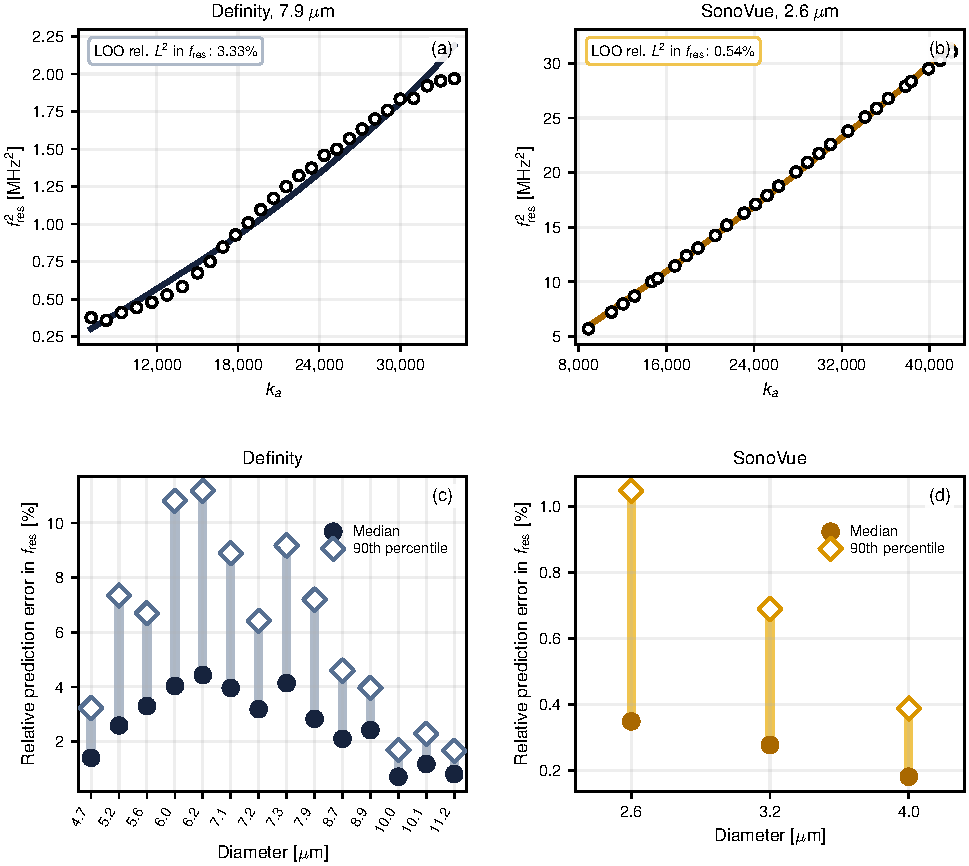
\includegraphics[width=0.98\linewidth]{Figure_6.pdf}
\caption{Polynomial acoustic surrogate validation. Panels (a) and (b) compare held-out squared \textsc{dpd} resonance frequencies with polynomial-surrogate predictions at representative diameters associated with retained acoustic measurements for Definity (ink) and SonoVue (gold), respectively; open circles denote held-out squared \textsc{dpd} resonance frequencies and solid lines denote surrogate predictions. Panels (c) and (d) summarize the leave-one-out relative errors in $f_{\mathrm{res}}$ at all diameters associated with retained acoustic measurements (Refs.~\cite{goertz2006pulse,vandermeer2004sonovue}); filled circles show the median and open diamonds show the $90^{th}$ percentile.}
\label{fig:polynomial_surrogate_validation}
\end{figure}

Fig.~\ref{fig:polynomial_surrogate_validation} shows that the diameter-specific relative $L^2$ errors in $f_{\mathrm{res}}$ range from 0.9--4.9\% for Definity and 0.3--0.5\% for SonoVue. These results support the use of the polynomial surrogates as acoustic surrogates in the subsequent hierarchical inference.


\label{sec:res:phase2}
\begin{figure}%[!htb]%[t]
\centering
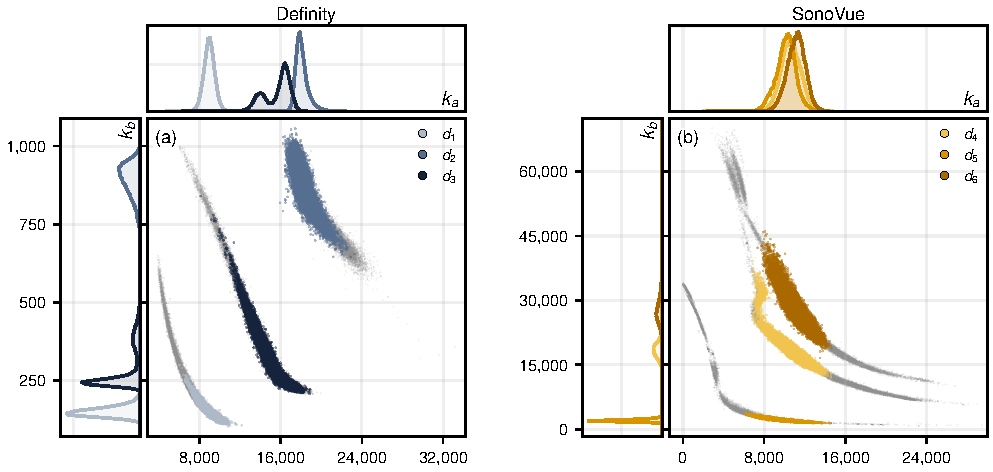
\includegraphics[width=\textwidth]{Figure_7.pdf}
\caption{Reduced-model posterior clouds from independent force spectroscopy inference and hierarchical inference conditioned jointly on force spectroscopy and acoustic data for the dominant elastic parameters $k_a$ and $k_b$. Each point denotes a posterior sample. The top and side marginal traces show the corresponding one-dimensional posterior densities for $k_a$ and $k_b$. Panel (a) corresponds to Definity \textsc{emb}s (ink), and panel (b) to SonoVue \textsc{emb}s (gold). Pale grey point clouds show regions compatible with the force spectroscopy data in the linear regime, while ink and gold point clouds show the hierarchical posteriors conditioned jointly on force spectroscopy and acoustic data for Definity and SonoVue, respectively.}
\label{fig:phase1_vs_phase3b_reduced_summary}
\end{figure}
For both Definity and SonoVue models, we then infer hierarchical hyperparameters for the reduced models to quantify how $(k_a, k_b, d_0)$ vary across diameters while conditioning on the mechanical and acoustic observations (Methods, sec.~\ref{sec:meth:bayes}). For each \textsc{emb} model, this step pools information across its three mechanically calibrated diameters and the acoustic observations to learn hierarchical priors that regularize the diameter-specific posteriors. Using these learned priors, we subsequently perform diameter-specific \textsc{tmcmc} inference for the three diameters of each \textsc{emb} model (see Fig.~\ref{fig:workflow}, block \textcircled{3}). For each bubble $i$, these posteriors $P(\tilde\theta_{d_i})$ constitute the reduced-model distributions used downstream for propagated-response bands, Maximum A Posteriori (\textsc{map}) extraction, and spectroscopy-only full-model consistency checks. Fig.~\ref{fig:phase1_vs_phase3b_reduced_summary} compares the broad regions compatible with the force spectroscopy data in the linear regime with hierarchical posteriors conditioned jointly on force spectroscopy and acoustic data in the $(k_a,k_b)$ plane. The hierarchical posteriors cover a substantially narrower part of the mechanical compatibility ridge while retaining diameter-specific structure within each \textsc{emb} model.

\begin{figure}%[!htb]%[t]
\centering
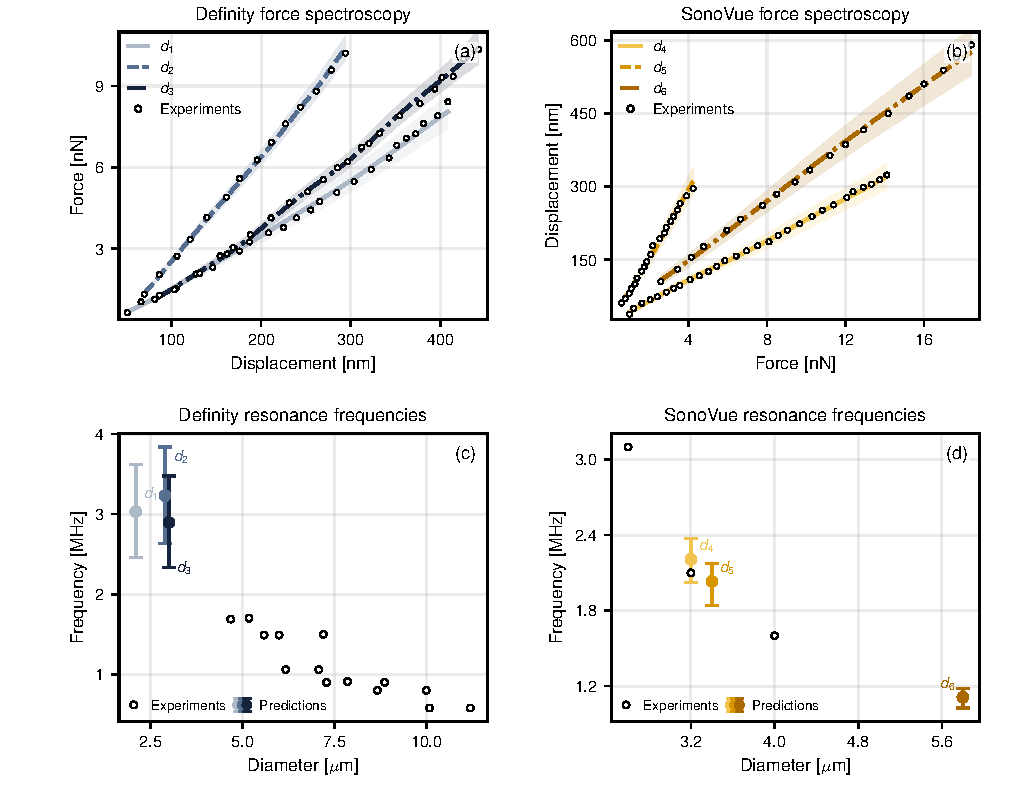
\includegraphics[width=\textwidth]{Figure_8.pdf}
\caption{Reduced-model posterior propagation. Panels (a) and (b) show Definity (ink) compression and SonoVue (gold) indentation responses, respectively, with all three diameters overlaid in each case. For each diameter, colored lines denote the reduced hierarchical posterior median response, shaded bands denote central 90\% posterior predictive intervals, and open circles denote force spectroscopy data in the retained linear regime. Panels (c) and (d) show posterior medians and intervals propagated through the acoustic surrogates together with acoustic observations shown as open circles. Experimental data are from Refs.~\cite{buchner2012,morris2014mechanical,vandermeer2004sonovue,goertz2006pulse}.}
\label{fig:reduced_bands_all}
\end{figure}
Fig.~\ref{fig:reduced_bands_all} shows that the jointly conditioned posteriors remain compatible with both the retained force spectroscopy data and the acoustic observations. In Fig.~\ref{fig:reduced_bands_all}(c), the available Definity frequency measurements concern bubbles larger than $d_1$--$d_3$, whereas the predictions are reported at $d_1$--$d_3$. The shared Definity hierarchy transfers this information to $d_1$--$d_3$ under the assumption that all Definity datasets arise from a common parameter population. No empirical frequency--diameter relation is fitted or extrapolated.

\label{sec:res:map_confirmation}

To confirm that the surrogate-based reduced calibrations remain faithful to the underlying particle-based model at representative reduced-model \textsc{map} parameter sets, we compare reduced-model \textsc{map} curves from \textsc{dnn}-guided inferences with direct \textsc{dpd} runs (see Fig.~\ref{fig:workflow}, block \textcircled{4}). Because propagating full posterior uncertainty directly through the \textsc{dpd} simulations would require prohibitively many expensive evaluations, we restrict the direct confirmation in the present paper to sparse \textsc{map}-level overlays. For both Definity and SonoVue models, the direct reduced-model \textsc{map} \textsc{dpd} responses compare well with the experimental force spectroscopy data in the linear regime. Fig.~\ref{fig:map_confirmation_reduced} displays these mechanical comparisons together with direct \textsc{dpd} resonance frequencies for all six bubbles.

\begin{figure}%[!htb]%[t]
\centering
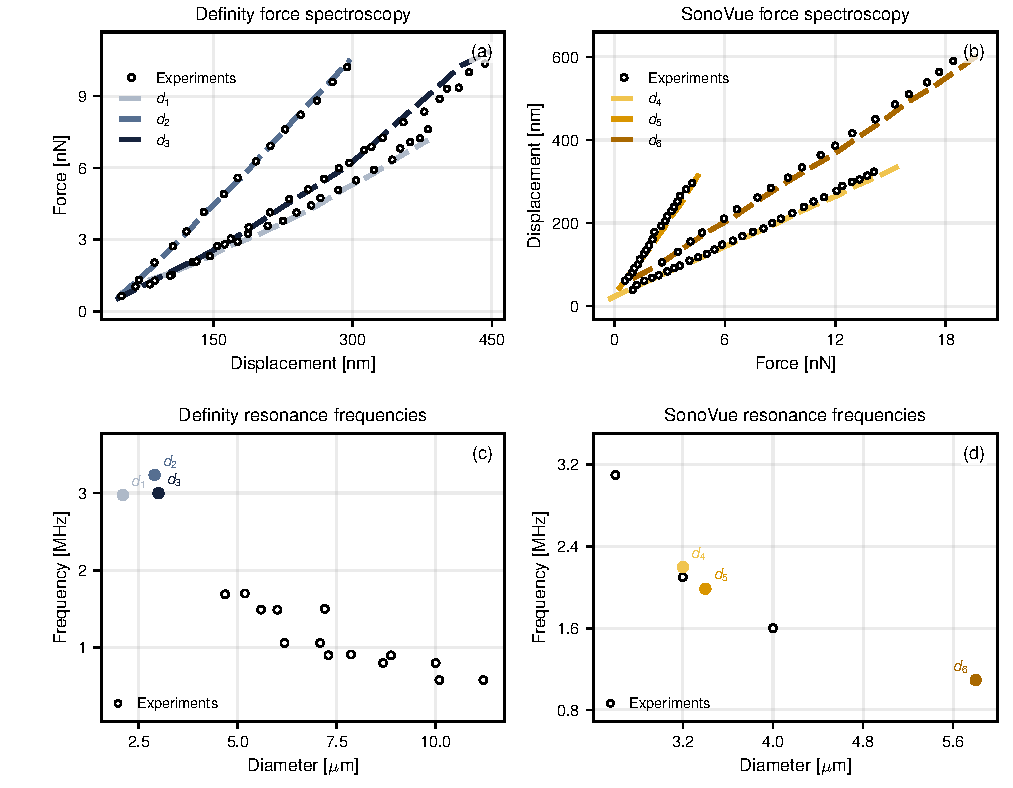
\includegraphics[width=\textwidth]{Figure_9.pdf}
\caption{Direct \textsc{dpd} consistency checks at the reduced-model \textsc{map} values for all six bubbles. Panels (a) and (b) compare force spectroscopy data in the linear regime with direct \textsc{dpd} responses for Definity (ink) and SonoVue (gold), respectively. Panels (c) and (d) compare acoustic observations with direct \textsc{dpd} resonance frequencies at the corresponding \textsc{map} values. Experimental data are from Refs.~\cite{buchner2012,morris2014mechanical,vandermeer2004sonovue,goertz2006pulse}.}
\label{fig:map_confirmation_reduced}
\end{figure}

The final reduced hierarchical \textsc{map} values of the dominant elastic parameters are summarized in Table~\ref{tab:map_parameters_reduced}.

\label{sec:res:reduced_model}
  
Separately from the acoustically conditioned reduced workflow, we retain the spectroscopy-only full-versus-reduced comparison as a sanity check on the reduced parameterization. In this comparison, the full and reduced force fields are calibrated to the same force spectroscopy data, and we quantify the discrepancy between their \textsc{map} surrogate responses via the relative $L^2$ difference, $100\lVert y_{\mathrm{full}}^{\mathrm{MAP}}-y_{\mathrm{red}}^{\mathrm{MAP}}\rVert_2/\lVert y_{\mathrm{full}}^{\mathrm{MAP}}\rVert_2$.
The worst-case discrepancy across diameters remains below 1.2\% for Definity and below 1.9\% for SonoVue. Fig.~\ref{fig:full_vs_reduced_map_overlay} compares the full- and reduced-model \textsc{map} surrogates in real units, showing that the two workflows are close at the level of the fitted response. This spectroscopy-only agreement is further supported by the \textsc{crps} \cite{matheson1976scoring,hersbach2000decomposition}, which measures how closely the full posterior predictive distribution matches the observed data while rewarding both calibration and sharpness, and shows comparable performance of the full and reduced models in terms of coverage and statistical consistency with the reference data (Tables S5 and S6 in the supplementary material). Together with the \textsc{map} overlays, these results show that the reduced and full force spectroscopy workflows have similar posterior-predictive \textsc{crps} values. We therefore use the full workflow here only as a confirmatory safety check. The practical conclusion is that, in the present quasi-static regime, the nonlinear elastic terms are weakly informed and the reduced model captures the dominant behavior in the linear regime that the data can support.

\begin{figure}%[!htb]%[t]
\centering
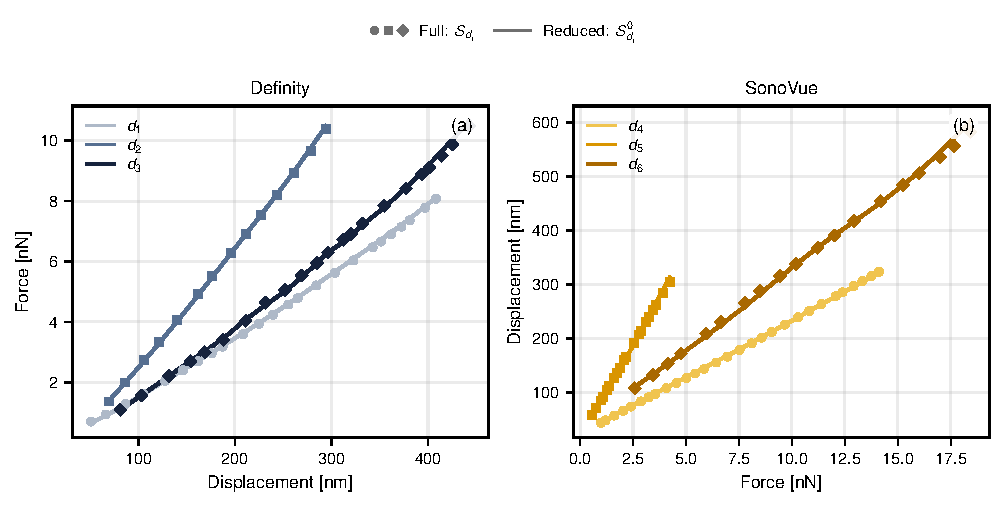
\includegraphics[width=\textwidth]{Figure_10.pdf}
\caption{Full- versus reduced-model surrogate sanity check. Panels (a) and (b) show Definity (ink) and SonoVue (gold), respectively. In both panels, the solid lines denote the reduced-model \textsc{map} surrogate responses, while the symbols denote the full-model \textsc{map} surrogate responses. The figure provides a direct \textsc{map}-level overlay check, showing that the full and reduced workflows are close in the present quasi-static regime.}
\label{fig:full_vs_reduced_map_overlay}
\end{figure}

\begin{table}
\caption{\label{tab:map_parameters_reduced}
Reduced hierarchical \textsc{map} values of the dominant elastic parameters
across different types and diameters.}
\begin{ruledtabular}
\scriptsize
\begin{tabular}{lccc}
Type & Diameter & $k_a$ & $k_b$ \\
\hline
& $d_1$ (2.1 $\mu$m) & 8,970.6 & 144.5 \\
Definity & $d_2$ (2.9 $\mu$m) & 17,786.1 & 926.9 \\
& $d_3$ (3.0 $\mu$m) & 16,594.4 & 241.6 \\
\hline
& $d_4$ (3.2 $\mu$m) & 10,657.5 & 18,326.8 \\
SonoVue & $d_5$ (3.4 $\mu$m) & 9,915.9 & 2,037.1 \\
& $d_6$ (5.8 $\mu$m) & 11,268.4 & 26,823.1 \\
\end{tabular}
\end{ruledtabular}
\end{table}

In both \textsc{emb} types, the stretching and bending responses dominate the observable force--displacement behavior, whereas the nonlinear coefficients remain only weakly constrained (Sections~\ref{sec:res:sensitivity} and \ref{sec:res:phase1}). That is why we adopted a reduced model immediately after the sensitivity analysis and retained the full model only for the spectroscopy sanity check in Sec.~\ref{sec:res:reduced_model}. This choice was later supported by stable reduced posteriors before and after hierarchical pooling, and close full-vs-reduced \textsc{map} overlays and posterior-predictive \textsc{crps}. This result implies that the nonlinear interactions are weakly constrained by the present experiments and do not significantly improve the fitted response in this regime. With the reduced parameterization fixed, the hierarchical inference step then serves to regularize reduced-model posteriors through population-level structure learned in the hyperparameter inference phase (Sec.~\ref{sec:res:phase2}).

As can be seen in Table~\ref{tab:map_parameters_reduced}, the inferred values of $k_a$ and $k_b$ differ across bubble diameters. This is not surprising since the microbubbles used in experiments differ in shell thickness, lipid packing and loading history. This is physically important because in the thin shell limit the in-plane elastic constants scale linearly with shell thickness, whereas the bending stiffness scales with the cube of the thickness. As a result even relatively small variations in the thickness can produce substantial differences in the effective mechanical response. The reported diameter dependent values of $k_a$ and $k_b$ should therefore be understood as effective coefficients describing each microbubble within the present modeling framework.

A separate source of uncertainty comes from curve alignment. In force--deformation measurements of \textsc{emb}, uncertainty in the precise location of first contact introduces a systematic ambiguity in the deformation coordinate. A calibrated quantity $d_0$ was therefore introduced to compensate for the initial loading state and alignment uncertainty in the reference curves, which are not explicitly represented in the present \textsc{dpd} model. It accounts for a real experimental ambiguity associated with contact-point determination and prevents that ambiguity from being attributed to shell stiffness. The scope of these conclusions is also limited by the experimental regime. The data are quasi-static and low dimensional, over a limited loading range, for six diameter-specific datasets. Validating the full force field would require additional observables, such as dynamic acoustic response. Finally, the uncertainty estimates are conditional on the surrogate pipeline. The workflow relies on surrogates constructed from finite simulation databases. The grouped-holdout \textsc{dnn} errors reported in Table S2 in the supplementary material and the leave-one-out polynomial errors reported in Fig.~\ref{fig:polynomial_surrogate_validation} are low enough to make the inference tractable and credible, but neither surrogate error is zero. In the current workflow, these surrogate errors are treated as zero during inference and propagation, so only parameter uncertainty and the inferred observation noise enter the displayed posterior predictive bands. A related limitation concerns direct simulation validation. The paper does not report posterior predictive bands computed directly with the underlying particle-based model itself: propagating a large posterior ensemble through \textsc{dpd} would be prohibitively expensive with the current simulation cost. Likewise, the direct \textsc{dpd} overlays reported in Results are representative \textsc{map}-level checks only; they are useful confirmation runs at selected parameter points, but not exhaustive validations over all diameters or over full posterior regions.

\section{Conclusion}

In this work, we developed data-informed \textsc{dpd} models that quantify the stretching stiffness and bending modulus of two types of lipid-\textsc{emb}s using a surrogate-accelerated Bayesian inference framework. Our models accounted for variations in \textsc{emb} size, elastic parameters, displacement offset, and measurement noise. Model parameters were calibrated against the linear regime of three force spectroscopy datasets for each \textsc{emb} type, together with acoustic-frequency observations entering the hierarchical calibration. The use of \textsc{dnn} mechanical surrogates and polynomial acoustic surrogates enabled efficient posterior sampling while maintaining high fidelity to the underlying \textsc{dpd} simulations. Parameter uncertainties were propagated through forward predictions to assess model robustness and transferability.

In addition to these uncertainties, the assumption of a constant membrane thickness introduces an additional source of uncertainty in the inferred elastic parameters. As noted in \textsc{afm} studies of phospholipid microbubbles, apparent variations in Young's modulus with \textsc{emb} size may arise from underlying variations in shell thickness, lipid packing or loading history, which can explain why the ordering of the reference experimental force--displacement curves does not necessarily follow the ordering of bubble diameter. To address this limitation, the \textsc{dpd} model could be extended to properly account for the variability of the shell-thickness, which could then be calibrated from the data. The next step, beyond the scope of the present quasi-static study, will be to test how the calibrated models perform in acoustic simulations. That setting would test dynamic behavior beyond the acoustic-frequency observations used here and would therefore help to assess whether the reduced force field remains sufficient beyond compression and indentation. Such studies would also show how calibration uncertainty in the mechanical parameters propagates to acoustically relevant predictions. If direct \textsc{dpd} uncertainty bands become necessary, one possible route would be to use an Unscented Transform built around a small set of carefully selected \textsc{dpd} evaluations~\cite{julier2002reduced}, so that uncertainty bands from \textsc{dpd} simulations can be approximated without brute-force posterior propagation. The more direct next step would be to carry the calibrated posterior distributions into acoustically relevant simulations and compare the resulting behavior across model choices. More broadly, this established surrogate-accelerated Bayesian route shows that rigorous \textsc{uq} for particle-based soft-matter models is feasible once high-fidelity simulations are coupled with surrogates and hierarchical Bayesian inference. This combination made it possible to calibrate parameters, compare reduced and full force fields, and identify weakly constrained terms. Even though the present study ultimately favored a reduced force field in this experimental regime, that outcome is still informative, because it identifies the level of model complexity supported by the current data and indicates what additional dynamic measurements and simulations would be needed to justify more complex models. Our force spectroscopy data-informed \textsc{emb} models provide a basis for large-scale acoustic simulations to determine key ultrasound parameters \cite{lah2025open}, such as intensity, pulse duration, and frequency for \textsc{usdg}. The methodology can be further extended to model development of ligand-functionalized \textsc{emb}s or encapsulated gas vesicles \cite{maresca2018biomolecular,salahshoor2022geometric,dutka2023structure,smith2025ultrafast,ntarakas2025dissipative}, and contrast agents for other imaging techniques including echocardiography \cite{kaufmann2007contrast}, magnetic resonance imaging, positron emission tomography, diffraction-enhanced X-ray imaging \cite{kogan2010microbubbles} and X-ray dark-field imaging \cite{velroyen2013microbubbles}.

\section*{Supplementary Material}
The supplementary material includes implementation details, experimental data information, hierarchical inference procedures, \textsc{tmcmc} and surrogate-model configurations, acoustic-frequency extraction, sensitivity-analysis methodology, and parameter tables.

\begin{acknowledgments}
The authors acknowledge financial support under the ERC Advanced Grant MULTraSonicA (Grant No.\,885155) from the European Research Council. We also acknowledge the EuroHPC Joint Undertaking for awarding the project ID EHPC-REG-2025R02-164 access to Vega at IZUM (Slovenia) and Karolina at e-INFRA CZ (Czech Republic). 
\end{acknowledgments}

\section*{Author Declarations}

\subsection*{Conflict of Interest}
The authors have no conflicts to disclose.

\subsection*{Author Contributions}

\textbf{Brieuc Benvegnen:} Investigation, Methodology, Software, Validation, Writing – original draft, Writing - review and editing.
\textbf{Nikolaos Ntarakas:} Investigation, Methodology, Software, Validation, Writing – original draft, Writing - review and editing.
\textbf{Tilen Potisk:} Investigation, Methodology, Software, Validation, Writing - review and editing.
\textbf{Ignacio Pagonabarraga:} Methodology, Supervision, Writing - review and editing.
\textbf{Matej Praprotnik:} Conceptualization, Funding acquisition, Methodology, Resources, Supervision, Writing - review and editing.



\section*{Data Availability}
The data used in this study is maintained in a private GitHub repository and will be made public upon publication.

\bibliography{refs}

\end{document}
